\documentclass[12pt,lettepaper]{article}
\usepackage{graphicx}
\usepackage{array}
\usepackage{geometry}
\geometry{a4paper, margin=1in}

\begin{document}

% Name and Contact Information
\begin{flushleft}
    \Huge \textbf{Rajib Mondal }
\end{flushleft}

\begin{flushright}
    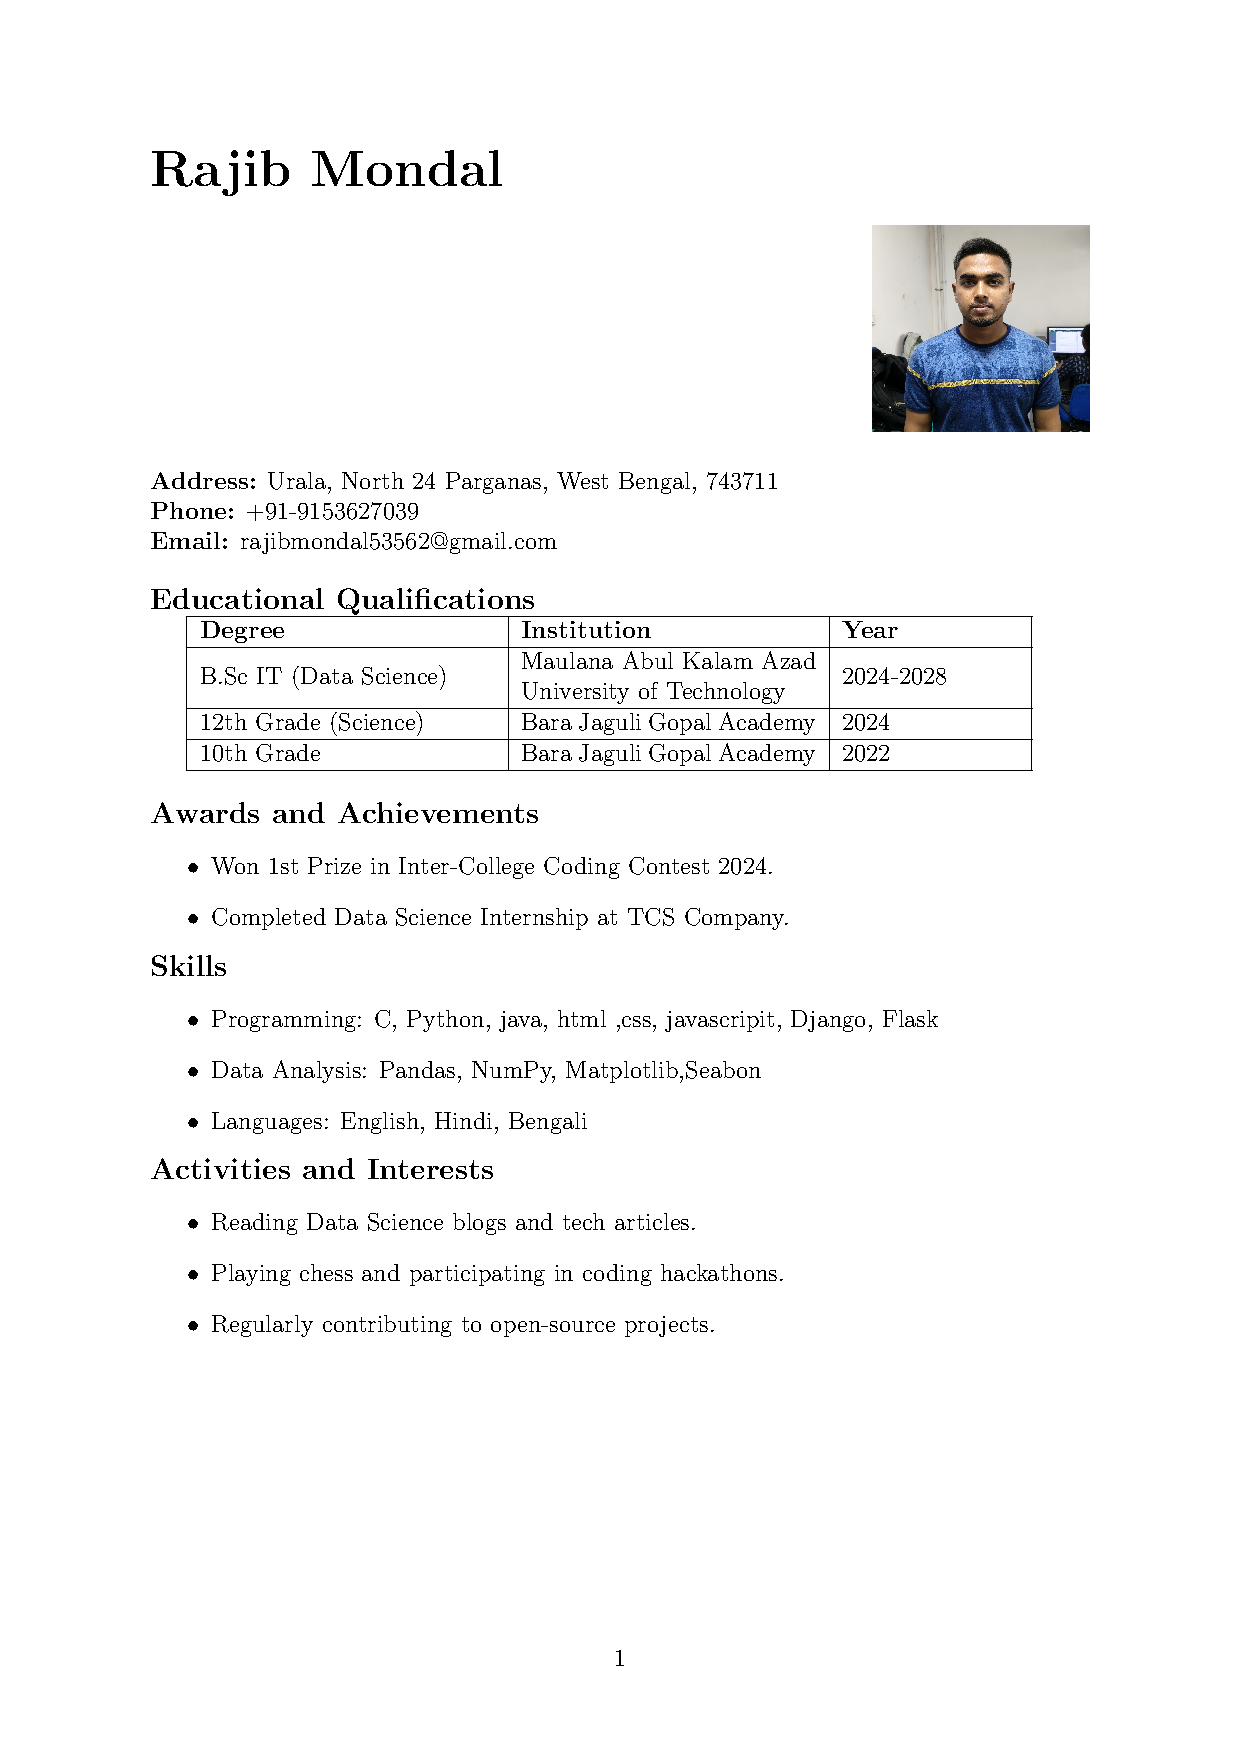
\includegraphics[width=3.7cm,height=3.5cm]{Rajib.jpeg}
\end{flushright}

\noindent
\textbf{Address:} Urala, North 24 Parganas, West Bengal, 743711 \\
\textbf{Phone:} +91-9153627039 \\
\textbf{Email:} rajibmondal53562@gmail.com

\vspace{0.5cm}

% Educational Qualifications
\noindent
\textbf{\large Educational Qualifications}

\begin{tabular}{| m{5cm} | m{5cm} | m{3cm} |}
    \hline
    \textbf{Degree} & \textbf{Institution} & \textbf{Year} \\
    \hline
    B.Sc IT (Data Science) & Maulana Abul Kalam Azad University of Technology & 2024-2028 \\
    \hline
    12th Grade (Science) & Bara Jaguli Gopal Academy & 2024 \\
    \hline
    10th Grade & Bara Jaguli Gopal Academy & 2022 \\
    \hline
\end{tabular}

\vspace{0.5cm}

% Awards and Achievements
\noindent
\textbf{\large Awards and Achievements}
\begin{itemize}
    \item Won 1st Prize in Inter-College Coding Contest 2024.
    \item Completed Data Science Internship at TCS Company.
\end{itemize}

% Skills
\noindent
\textbf{\large Skills}
\begin{itemize}
    \item Programming: C, Python, java, html ,css, javascripit, Django, Flask
    \item Data Analysis: Pandas, NumPy, Matplotlib,Seabon  
    \item Languages: English, Hindi, Bengali
\end{itemize}

% Activities and Interests
\noindent
\textbf{\large Activities and Interests}
\begin{itemize}
    \item Reading Data Science blogs and tech articles.
    \item Playing chess and participating in coding hackathons.
    \item Regularly contributing to open-source projects.
\end{itemize}

\end{document}
